%%%%%%%%%%%%%%%%%%%%%%%%%%%%%%%%%%%%%%%%%%%%%%%%%%%%%%%%%
\begin{frame}{변환이란}

수학적 의미에서 변환(transformation)

\begin{itemize}
\item 어떤 집합 $S$를 다른 어떤 집합 $S$로 대응시키는 함수
\item 공간과 점, 그리고 벡터의 문제로 이해할 때, 변환이란 공간 상의 벡터나 점을 다른 벡터나 점으로 바꾸는 연산
\item 변환 행렬
	\begin{itemize}
	\item 어떤 벡터 $\mathbf a$가 $\mathbb R^{n}$에 속한다고 할 때, 이 벡터에 행렬 $\mathbf A \in \mathbb R^{n \times n}$을 곱하면 $\mathbf a$와 같은 차원의 벡터 $\mathbf b$를 얻는다.
	\item $\mathbf b = \mathbf A \mathbf a ~ (\mathbf a, \mathbf b \in \mathbb R^n , \mathbf A \in \mathbb R^{n \times n})$.
	\item 어떤 벡터를 동일한 차원의 다른 벡터로 옮기는 행렬 $\mathbf A \in \mathbb R^{n \times n}$을 변환행렬(transform matrix)라고 한다.
	\end{itemize}
\end{itemize}

\end{frame}
%%%%%%%%%%%%%%%%%%%%%%%%%%%%%%%%%%%%%%%%%%%%%%%%%%%%%%%%%

%%%%%%%%%%%%%%%%%%%%%%%%%%%%%%%%%%%%%%%%%%%%%%%%%%%%%%%%%
\begin{frame}{좌표계 - 직교 좌표계}

\begin{itemize}
\item 일반적으로 가장 익숙한 좌표계
\item 데카르트 좌표계(Cartesian coordinate system)
\end{itemize}

\begin{figure}
    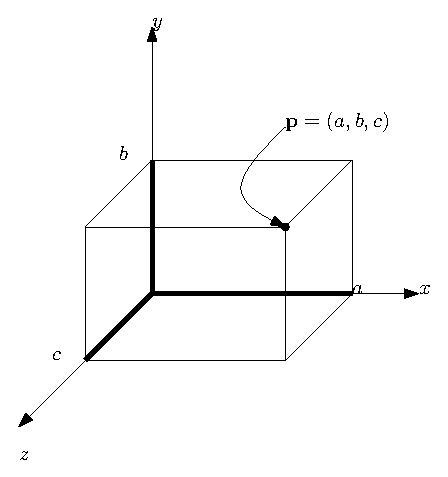
\includegraphics[width=6cm]{Math_transform/CartesianCoord.eps}
\end{figure}

\end{frame}
%%%%%%%%%%%%%%%%%%%%%%%%%%%%%%%%%%%%%%%%%%%%%%%%%%%%%%%%%

%%%%%%%%%%%%%%%%%%%%%%%%%%%%%%%%%%%%%%%%%%%%%%%%%%%%%%%%%
\begin{frame}{좌표계 - 원기둥 좌표계}

\begin{itemize}
\item $\mathbf p$는 이러한 높이 $h$와 반지름 $r$을 가진 원기둥의 윗쪽 원주에 놓임.
\item 원주에서 특정한 위치는 각도 $\theta$로 표현
\item 원기둥 좌표: $(r, \theta, h)$
\end{itemize}

\begin{figure}
    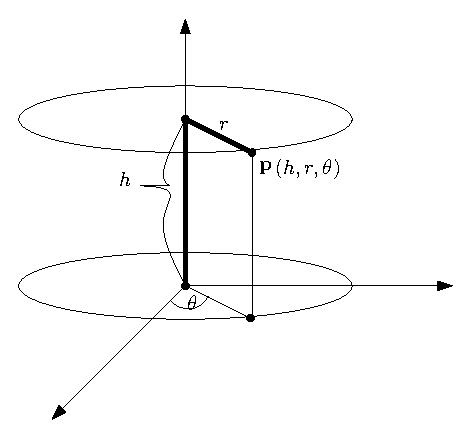
\includegraphics[width=6.5cm]{Math_transform/cylindricCoord.eps}
\end{figure}

\end{frame}
%%%%%%%%%%%%%%%%%%%%%%%%%%%%%%%%%%%%%%%%%%%%%%%%%%%%%%%%%

%%%%%%%%%%%%%%%%%%%%%%%%%%%%%%%%%%%%%%%%%%%%%%%%%%%%%%%%%
\begin{frame}{원기둥 좌표를 직교 좌표로 옮기기}

원기둥 좌표계의 좌표를 $\mathbf p_{cyl}$, 직교 좌표계의 좌표를 $\mathbf p_{cart}$으로 표현하면

$$(r, \theta, h)_{cyl} = ( r \cos \theta , r \sin \theta, h)_{cart}$$

\begin{figure}[h!]
  \centering
    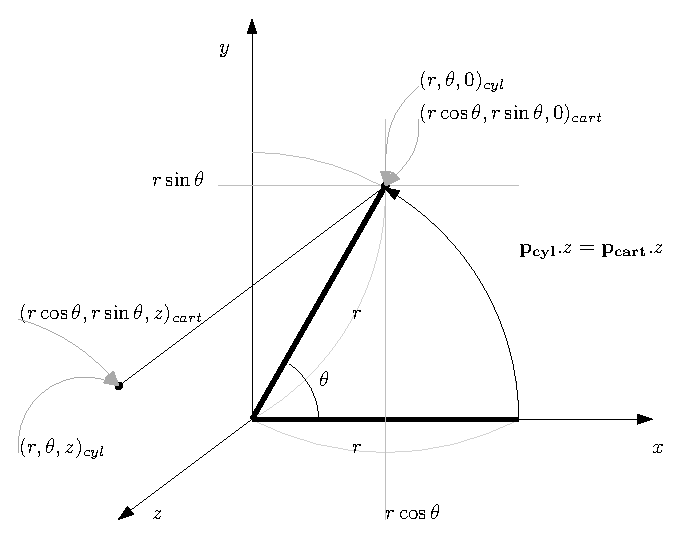
\includegraphics[width=6.5cm]{Math_transform/cyl2Cartesian.eps}
\end{figure}

\end{frame}
%%%%%%%%%%%%%%%%%%%%%%%%%%%%%%%%%%%%%%%%%%%%%%%%%%%%%%%%%


%%%%%%%%%%%%%%%%%%%%%%%%%%%%%%%%%%%%%%%%%%%%%%%%%%%%%%%%%
\begin{frame}{좌표계 - 구면 좌표계}

\begin{itemize}
\item $\mathbf p$를 지나며 중심이 원점인 구면의 반지름을 $r$
\item 반지름 $r$인 점 가운데  $x$ 축 위에 있는 점을 $\mathbf p_x$
\item $\mathbf p_x$을 $xy$ 평면 위에서 $\mathbf p$와 같은 경도선에 놓는 각도가 $\phi$
\item 이를 들어 올려 점 $\mathbf p$를 지나도록 하는 데에 필요한 각도를 $\theta$
\item 구면 좌표 $(r, \theta, \phi)$
\end{itemize}

\begin{figure}
    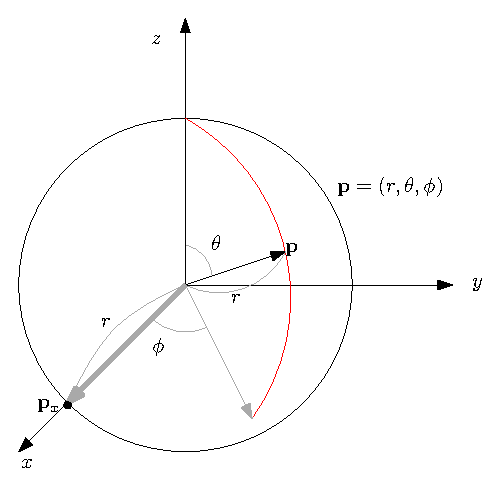
\includegraphics[width=5cm]{Math_transform/sphericalCoord.eps}
\end{figure}

\end{frame}
%%%%%%%%%%%%%%%%%%%%%%%%%%%%%%%%%%%%%%%%%%%%%%%%%%%%%%%%%

%%%%%%%%%%%%%%%%%%%%%%%%%%%%%%%%%%%%%%%%%%%%%%%%%%%%%%%%%
\begin{frame}{구면 좌표와 직교 좌표}

{\small
구면 좌표는 일반적으로 다음과 같은 제한을 갖는다.
$$r \geq 0$$
$$0 \leq \theta \leq \pi$$
$$0 \leq \phi \leq 2 \pi $$

직교 좌표계의 좌표 $(x,y,z)$를 구면 좌표계로 옮기기

\begin{eqnarray}
r &= \sqrt{x^2 + y^2 + z^2} \nonumber \\
\theta & = \arccos \left ( \frac{z}{\sqrt{x^2 + y^2 + z^2}} \right ) \nonumber \\
\phi &= \arctan \left ( \frac{y}{x} \right ) \nonumber
\end{eqnarray}

구면 좌표계의 좌표를 직교 좌표로 옮기기

\begin{eqnarray}
x &= r \sin \theta \cos \phi \nonumber \\
y & = r \sin \theta \sin \phi \nonumber \\
z & =r \cos \theta \nonumber
\end{eqnarray}
}

\end{frame}
%%%%%%%%%%%%%%%%%%%%%%%%%%%%%%%%%%%%%%%%%%%%%%%%%%%%%%%%%

%%%%%%%%%%%%%%%%%%%%%%%%%%%%%%%%%%%%%%%%%%%%%%%%%%%%%%%%%
\begin{frame}{무슨 좌표계를 사용할 것인가}

\begin{itemize}
\item 공간에 존재하는 점을 다룰 때에는 어떠한 좌표계를 사용해도 무방
\item 컴퓨터 그래픽스 분야에서 가장 많이 사용되는 좌표계는 직교 좌표계
\item 우리는 직교 좌표계에서 변환에 대해 다룰 예정
\item 직교 좌표계를 기본적인 좌표계로 삼고 변환과 관련된 행렬 연산을 살필 것
\end{itemize}

\end{frame}
%%%%%%%%%%%%%%%%%%%%%%%%%%%%%%%%%%%%%%%%%%%%%%%%%%%%%%%%%


%%%%%%%%%%%%%%%%%%%%%%%%%%%%%%%%%%%%%%%%%%%%%%%%%%%%%%%%%
\begin{frame}{어파인(affine) 변환}

{\small
게임을 구현하기 위한 3차원 그래픽스에서 흔히 사용되는 변환

\begin{itemize}
\item 이동변환(translation): 주어진 변위 벡터만큼 좌표를 동일하게 옮김
\item 회전변환(rotation): 2차원은 기준점, 3차원은 기준축을 중심으로 돌림
\item 크기변경(scaling): 각 축 방향으로 주어진 비율에 따라 좌표 값이 커지거나 줄어든다.
\end{itemize}

이러한 변환은 어파인 변환(affine transformation)의 일종
\begin{itemize}
\item 서로 연결되어 있음을 의미하는 라틴어 `affinis'에서 유래
\item 직선 위의 점들을 직선을 유지한 상태로 변환하는 변환
\item 직선 위에서의 점들 사이의 거리 비가 변환된 직선 위에서 그대로 유지
\item 직선은 직선으로, 평행선은 평행선으로 유지
\item 실시간 컴퓨터 그래픽스에서는 여러 가지 효율성의 이유로 어파인 변환을 사용
\end{itemize}
}

\end{frame}
%%%%%%%%%%%%%%%%%%%%%%%%%%%%%%%%%%%%%%%%%%%%%%%%%%%%%%%%%


%%%%%%%%%%%%%%%%%%%%%%%%%%%%%%%%%%%%%%%%%%%%%%%%%%%%%%%%%
\begin{frame}{이동 변환(translation)}

{\small
\begin{itemize}
\item 2차원: 좌표 $(x,y)$를 $x$ 축 방향으로 $a$, $y$ 축 방향으로 $b$ 만큼 옮기기
\item $(x', y') = (x,y) + (a,b) = (x+a, y+a)$
\end{itemize}

\begin{itemize}
\item 모든 차원에 대해
어떤 벡터 $\mathbf a$를 변위 벡터 $\mathbf d$를 이용하여 $\mathbf x'$로 옮기는 이동 변환을 다음과 같이 벡터 더하기로 정의할 수 있음
	\begin{itemize}
	\item $\mathbf a \in \mathbb R^n, \mathbf d \in \mathbb R^n$
	\item $\mathbf x' = \mathbf a + \mathbf d~~~~\mathbf x' \in \mathbb R^n$
	\end{itemize}
\end{itemize}


\begin{figure}
    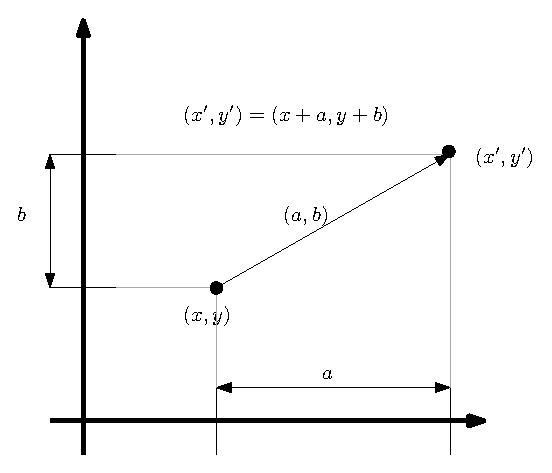
\includegraphics[width=5cm]{Math_transform/translation.eps}
\end{figure}
}

\end{frame}
%%%%%%%%%%%%%%%%%%%%%%%%%%%%%%%%%%%%%%%%%%%%%%%%%%%%%%%%%


%%%%%%%%%%%%%%%%%%%%%%%%%%%%%%%%%%%%%%%%%%%%%%%%%%%%%%%%%
\begin{frame}{2차원 회전 변환(rotation) - 문제}

{\small
\begin{itemize}
\item 2차원 회전의 중심: 피벗(pivot)
\item 기본적인 회전: 피벗이 원점인 경우
	\begin{itemize}
	\item $\mathbf p$를 원점을 중심으로 $\theta$ 만큼 회전하여 놓이는 지점 $\mathbf p'$를 구하는 문제
	\item 원래 좌표 $(p_x,p_y)$를 $\theta$ 만큼 회전하여 얻는 $(p'_x, p'_y)$를 얻는 문제
	\end{itemize}
\end{itemize}

\begin{figure}
    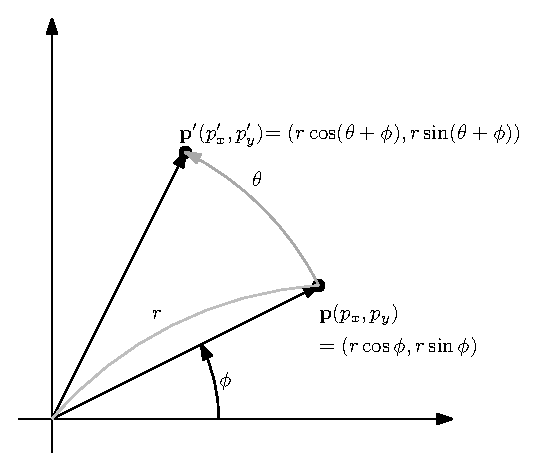
\includegraphics[width=6cm]{Math_transform/rotation.eps}
\end{figure}


}

\end{frame}
%%%%%%%%%%%%%%%%%%%%%%%%%%%%%%%%%%%%%%%%%%%%%%%%%%%%%%%%%


%%%%%%%%%%%%%%%%%%%%%%%%%%%%%%%%%%%%%%%%%%%%%%%%%%%%%%%%%
\begin{frame}{2차원 회전 변환(rotation) - 좌표값에 대한 이해}

\begin{figure}
    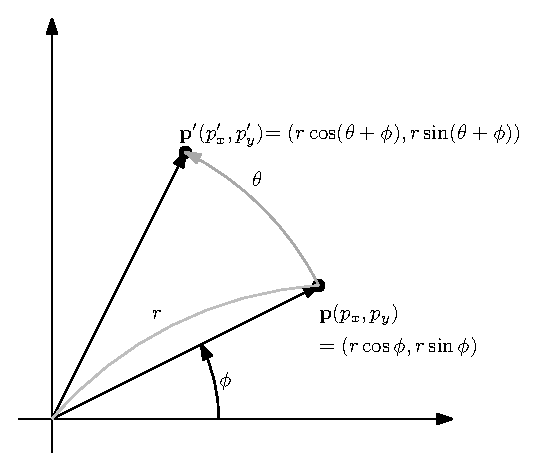
\includegraphics[width=5cm]{Math_transform/rotation.eps}
\end{figure}

\begin{itemize}
\item 원점에서 $(p_x,p_y)$로 선분: 선분 길이 $r$과 $x$축과 이루는 각도 $\phi$
\item $(p_x, p_y) = (r \cos \phi,  r \sin \phi)$
\item 이 좌표를 $\theta$만큼 회전하여 얻는 $(p'_x , p'_y)$
	\begin{itemize}
	\item $(p'_x, p'_y) =  ( r \cos (\theta+ \phi) , r \sin (\theta + \phi) )$
	\end{itemize}
\end{itemize}

\end{frame}
%%%%%%%%%%%%%%%%%%%%%%%%%%%%%%%%%%%%%%%%%%%%%%%%%%%%%%%%%


%%%%%%%%%%%%%%%%%%%%%%%%%%%%%%%%%%%%%%%%%%%%%%%%%%%%%%%%%
\begin{frame}{2차원 회전 변환(rotation) - 회전결과}

\begin{itemize}
\item $\phi$를 계산하지 않고 답을 얻어야 함
\item 참조할 공식
	\begin{itemize}
	\item $\cos (a+b) = \cos a \cos b - \sin a \sin b$
	\item $\sin (a+b) = \sin a \cos b + \cos a \sin b$
	\end{itemize}
\item 회전하여 얻는 좌표는 다음과 같이 표현
	\begin{itemize}
	\item $p'_x = (r \cos \phi) \cos \theta - (r \sin \phi )\sin \theta$
	\item $p'_y = (r \cos \phi) \sin \theta + (r \sin \phi )\cos \theta$
	\end{itemize}
\item 원래의 좌표 $(p_x , p_y )$를 이용하여 표현
	\begin{itemize}
	\item $p'_x = p_x \cos \theta - p_y \sin \theta$
	\item $p'_y = p_x \sin \theta + p_y \cos \theta$
	\end{itemize} 
\end{itemize}



\end{frame}
%%%%%%%%%%%%%%%%%%%%%%%%%%%%%%%%%%%%%%%%%%%%%%%%%%%%%%%%%

%%%%%%%%%%%%%%%%%%%%%%%%%%%%%%%%%%%%%%%%%%%%%%%%%%%%%%%%%
\begin{frame}{2차원 회전 변환(rotation) - 행렬표현}

이러한 변환은 다음과 같은 행렬과 벡터의 곱으로 표현할 수 있다.

\begin{eqnarray}
\left [
\begin{array}{c}
p'_x \\ p'_y
\end{array}
\right ] =
\left [
\begin{array}{cc}
\cos \theta & - \sin \theta \\
\sin \theta & \cos \theta
\end{array}
\right ]
\left [
\begin{array}{c}
p_x \\
p_y
\end{array}
\right ] \nonumber
\end{eqnarray}

2차원 공간에서 어떤 점 $\mathbf p$를 원점 기준으로 $\theta$만큼 회전시켜 $\mathbf p'$를 얻는 변환은 회전변환 행렬 $\mathbf R(\theta)$을
이용하여 $\mathbf p' = \mathbf R(\theta) \mathbf p$로 표현할 수 있다.

\begin{eqnarray}
\mathbf R(\theta) = \left [ 
\begin{array}{cc}
\cos \theta & - \sin \theta \\
\sin \theta & \cos \theta
\end{array}
\right ] \nonumber
\end{eqnarray} 

\end{frame}
%%%%%%%%%%%%%%%%%%%%%%%%%%%%%%%%%%%%%%%%%%%%%%%%%%%%%%%%%


%%%%%%%%%%%%%%%%%%%%%%%%%%%%%%%%%%%%%%%%%%%%%%%%%%%%%%%%%
\begin{frame}[fragile]{3차원 회전 - $z$ 축 회전}

\begin{itemize}
\item 2차원 회전을 그대로 3차원에 적용
	\begin{itemize}
	\item 3차원 좌표 $\mathbf p = (p_x, p_y, p_z)$을 $z$ 기준으로 회전
	\end{itemize}
\item 이 변환은 2차원 변환에 $z$ 성분만 추가
	\begin{itemize}
	\item $z$ 축 성분은 그대로 유지된다. ($p'_z = p_z)$
	\item $p_x, p_y$의 값은 2차원 회전과 동일하게 변환된다.
	\end{itemize}
\end{itemize}

\begin{eqnarray}
\begin{array}{clrrr} 
p'_x  & = &\cos \theta \cdot p_x &- \sin \theta \cdot p_y &+ 0 \cdot p_z \\
p'_y  & = &\sin \theta \cdot p_x &+ \cos \theta \cdot p_y &+ 0 \cdot p_z \\
p'_z  & = & 0 \cdot p_x &+ 0 \cdot p_y &+ 1 \cdot p_z
\end{array} \nonumber
\end{eqnarray}

이것은 다음과 같은 행렬 표현으로 다시 쓸 수 있다.

\begin{eqnarray}
\left [ \begin{array}{c} p'_x \\ p'_y \\ p'_z  \end{array} \right ] 
=
\left [ \begin{array}{rrr}
\cos \theta &- \sin \theta  & 0  \\
\sin \theta & \cos \theta  & 0 \\
0 & 0  & 1 
\end{array} \right ]
\left [ \begin{array}{c} p_x \\ p_y \\ p_z \end{array} \right ]  \nonumber
\end{eqnarray}


\end{frame}
%%%%%%%%%%%%%%%%%%%%%%%%%%%%%%%%%%%%%%%%%%%%%%%%%%%%%%%%%


%%%%%%%%%%%%%%%%%%%%%%%%%%%%%%%%%%%%%%%%%%%%%%%%%%%%%%%%%
\begin{frame}{3차원 회전 - $y$ 축 회전 (1/2)}

\begin{figure}
    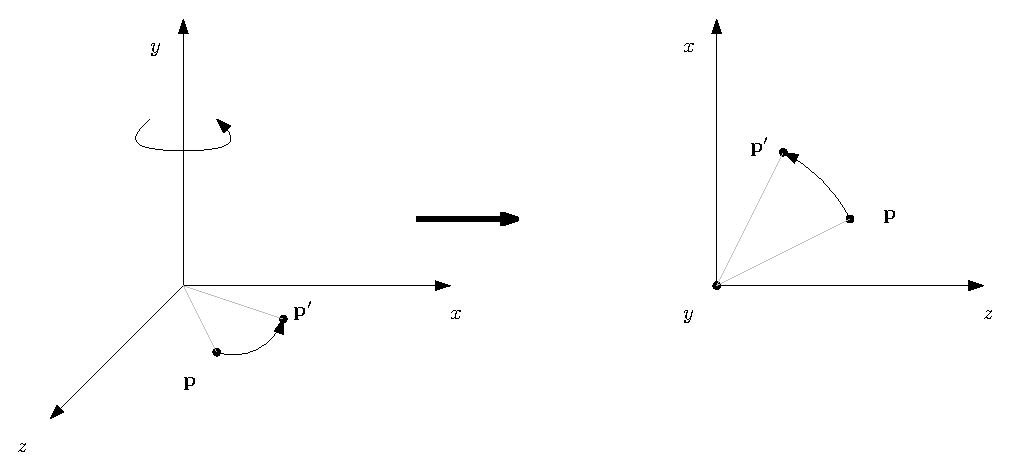
\includegraphics[width=10cm]{Math_transform/yAxisRotation.eps}
\end{figure}

\begin{itemize}
\item $z$ 축은 2차원 회전의 $x$축에 대응
\item $x$ 축은 2차원 회전의 $y$축에 대응
\end{itemize}

\begin{eqnarray}
\begin{array}{clrrr}
p'_z  & = &\cos \theta \cdot p_z &- \sin \theta \cdot p_x &+ 0 \cdot p_y \\
p'_x  & = &\sin \theta \cdot p_z &+ \cos \theta \cdot p_x &+ 0 \cdot p_y \\
p'_y  & = & 0 \cdot p_z &+ 0 \cdot p_x &+ 1 \cdot p_y
\end{array} \nonumber
\end{eqnarray}


\end{frame}
%%%%%%%%%%%%%%%%%%%%%%%%%%%%%%%%%%%%%%%%%%%%%%%%%%%%%%%%%


%%%%%%%%%%%%%%%%%%%%%%%%%%%%%%%%%%%%%%%%%%%%%%%%%%%%%%%%%
\begin{frame}{3차원 회전 - $y$ 축 회전 (1/2)}

순서를 재배열하면 다음과 같은 식을 얻는다.

\begin{eqnarray}
\begin{array}{clrrr}
p'_x  & = & \cos \theta \cdot p_x &+ 0 \cdot p_y &+ \sin \theta \cdot p_z  \\
p'_y  & =  &0 \cdot p_x &+ 1 \cdot p_y & 0 \cdot p_z \\
p'_z  & = &-\sin \theta \cdot p_x &+ 0 \cdot p_y  & + \cos \theta \cdot p_z 
\end{array} \nonumber
\end{eqnarray}

이것도 역시 행렬 표현으로 다시 쓸 수 있다.

\begin{eqnarray}
\left [ \begin{array}{c} p'_x \\ p'_y \\ p'_z  \end{array} \right ] 
=
\left [ \begin{array}{rrr}
\cos \theta & 0 &  \sin \theta  \\
0 & 1 & 0 \\
- \sin \theta & 0 & \cos \theta
\end{array} \right ]
\left [ \begin{array}{c} p_x \\ p_y \\ p_z \end{array} \right ]  \nonumber
\end{eqnarray}


\end{frame}
%%%%%%%%%%%%%%%%%%%%%%%%%%%%%%%%%%%%%%%%%%%%%%%%%%%%%%%%%

%%%%%%%%%%%%%%%%%%%%%%%%%%%%%%%%%%%%%%%%%%%%%%%%%%%%%%%%%
\begin{frame}{3차원 회전 - $x$ 축 회전 (1/2)}

\begin{itemize}
\item 2차원 회전에서 $x$, $y$의 역할에 $y$와 $z$ 축이 각각 대응
\end{itemize}

\begin{figure}
    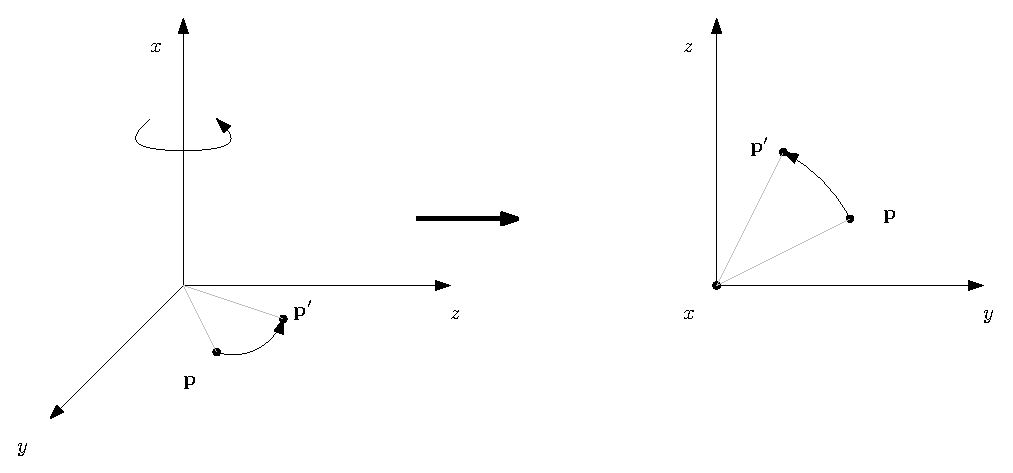
\includegraphics[width=10cm]{Math_transform/xAxisRotation.eps}
\end{figure}

\begin{eqnarray}
\begin{array}{clrrr}
p'_y  & = &\cos \theta \cdot p_y &- \sin \theta \cdot p_z &+ 0 \cdot p_x \\
p'_z  & = &\sin \theta \cdot p_y &+ \cos \theta \cdot p_z &+ 0 \cdot p_x \\
p'_x  & = & 0 \cdot p_y &+ 0 \cdot p_z &+ 1 \cdot p_x
\end{array} \nonumber
\end{eqnarray}


\end{frame}
%%%%%%%%%%%%%%%%%%%%%%%%%%%%%%%%%%%%%%%%%%%%%%%%%%%%%%%%%

%%%%%%%%%%%%%%%%%%%%%%%%%%%%%%%%%%%%%%%%%%%%%%%%%%%%%%%%%
\begin{frame}{3차원 회전 - $x$ 축 회전 (2/2)}

행렬과 벡터의 곱으로 표현하면 다음과 같다.

\begin{eqnarray}
\left [ \begin{array}{c} p'_x \\ p'_y \\ p'_z  \end{array} \right ] 
=
\left [ \begin{array}{rrr}
1 & 0 & 0 \\
0 & \cos \theta & - \sin \theta \\
0 & \sin \theta & \cos \theta
\end{array} \right ]
\left [ \begin{array}{c} p_x \\ p_y \\ p_z \end{array} \right ]  \nonumber
\end{eqnarray}

\end{frame}
%%%%%%%%%%%%%%%%%%%%%%%%%%%%%%%%%%%%%%%%%%%%%%%%%%%%%%%%%

%%%%%%%%%%%%%%%%%%%%%%%%%%%%%%%%%%%%%%%%%%%%%%%%%%%%%%%%%
\begin{frame}{회전 행렬의 역행렬}

\begin{itemize}
\item 회전행렬은 특별한 특징을 지님 (2차원 회전행렬을 보자)
	\begin{itemize}
	\item 첫 열 벡터는 길이는 $\sqrt{ \cos^2 \theta + \sin^2 \theta}$이므로 1
	\item 두 번째 열의 길이 역시 $\sqrt{ \sin^2 \theta + \cos^2 \theta}$로 1
	\item 즉 두 벡터 모두 단위 벡터 (정규)
	\item 이 두 벡터를 서로 내적하면 $\cos \theta ( - \sin \theta) + \sin \theta  \cos \theta $로 0
	\item 두 벡터가 서로 수직 (직교)
	\end{itemize}
\item 모든 벡터는 단위 벡터이고 서로 직교 = 정규직교(orthonormal)
\item 정규직교 행렬의 역행렬은 그 행렬의 전치(transpose)와 같음
\item 3차원 회전행렬들도 정규직교임을 쉽게 확인 가능
\end{itemize}

$${{\mathbf R}_x}^{-1}(\theta) = {{\mathbf R}_x}^{\rm T}(\theta)$$
$${{\mathbf R}_y}^{-1}(\theta) = {{\mathbf R}_y}^{\rm T}(\theta)$$
$${{\mathbf R}_z}^{-1}(\theta) = {{\mathbf R}_z}^{\rm T}(\theta)$$

\end{frame}
%%%%%%%%%%%%%%%%%%%%%%%%%%%%%%%%%%%%%%%%%%%%%%%%%%%%%%%%%

%%%%%%%%%%%%%%%%%%%%%%%%%%%%%%%%%%%%%%%%%%%%%%%%%%%%%%%%%
\begin{frame}{임의의 축에 대한 회전}

\begin{itemize}
\item 임의의 회전축을 기준으로  $\theta$만큼 회전하는 변환은 다음과 같은 절차를 따라 구현할 수 있다.

	\begin{enumerate}
	\item 회전축이 원점을 지나도록 이동변환 $\mathbf T$를 적용한다.
	\item 원점을 지나는 회전축이 $xz$ 평면에 놓이도록 $z$축 회전 $\mathbf R_1$ 적용
	\item 이 회전축이 $z$축과 동일한 방향이 되도록 $y$축 회전 $\mathbf R_2$를 적용한다.
	\item $z$축을 기준으로 $\theta$만큼 회전하도록 $\mathbf R_z(\theta)$를 적용한다.
	\item ${\mathbf R_2}^{-1}$, 즉 ${\mathbf R_2}^{\rm T}$를 적용한다.
	\item ${\mathbf R_1}^{-1}$, 즉 ${\mathbf R_1}^{\rm T}$를 적용한다.
	\item $\mathbf T^{-1}$, 즉 $- \mathbf T$를 적용한다.
	\end{enumerate}

\item 벡터 더하기(이동변환)와 행렬 곱하기(회전)가 혼재
\item 동차좌표계(homogeneous coordinate)을 이용
	\begin{itemize}
	\item 이동 변환과 회전 변환 모두 $4 \times 4$ 행렬
	\item 위의 절차를 모두 누적한 하나의 행렬로 표현 가능
	\end{itemize}
\item $\mathbf R_{pivot}(\theta) = - \mathbf T {\mathbf R_1}^{\rm T} {\mathbf R_2}^{\rm T}  \mathbf R_z(\theta) \mathbf R_2  \mathbf R_1 \mathbf T $
\end{itemize}


\end{frame}
%%%%%%%%%%%%%%%%%%%%%%%%%%%%%%%%%%%%%%%%%%%%%%%%%%%%%%%%%


%%%%%%%%%%%%%%%%%%%%%%%%%%%%%%%%%%%%%%%%%%%%%%%%%%%%%%%%%
\begin{frame}{동차좌표계(homogeneous coordinate)}

\begin{itemize}
\item 사영기하학(射影幾何學, projective geometry)에서 사용되는 좌표계
\item $n$ 차원의 사영공간을 $n+1$의 좌표로 표현
\item 그래픽 API나 라이브러리들은 동차좌표계를 표준적인 좌표계로 채용
	\begin{itemize}
	\item 3차원 그래픽스에서 정의된 3차원 가상 공간 객체의 2차원 투영 이미지를 얻는 일과 유관
	\item 3차원 공간의 어파인(affine) 변환들을 모두 $4 \times 4$의 행렬로 표현
	\end{itemize}
\item 3차원 공간의 좌표를 표현하는 벡터 $[x,y,z]^{\rm T}$는 동차좌표계에서 $[x,y,z,1]^{\rm T}$로 표현할 수 있음
\item 보다 일반적인 형태는 마지막 숫자를 1이 아닌 다른 값게 하는 것
\item 2차원: $[x,y,w]^{\rm T}$, 3차원: $[x,y,z,w]^{\rm T}$
\end{itemize}

\end{frame}
%%%%%%%%%%%%%%%%%%%%%%%%%%%%%%%%%%%%%%%%%%%%%%%%%%%%%%%%%


%%%%%%%%%%%%%%%%%%%%%%%%%%%%%%%%%%%%%%%%%%%%%%%%%%%%%%%%%
\begin{frame}{동차좌표계의 시각적 이해 (1/2)}

동차좌표계 이해를 위해 Ammeraal이 사용한 그림

\begin{figure}
    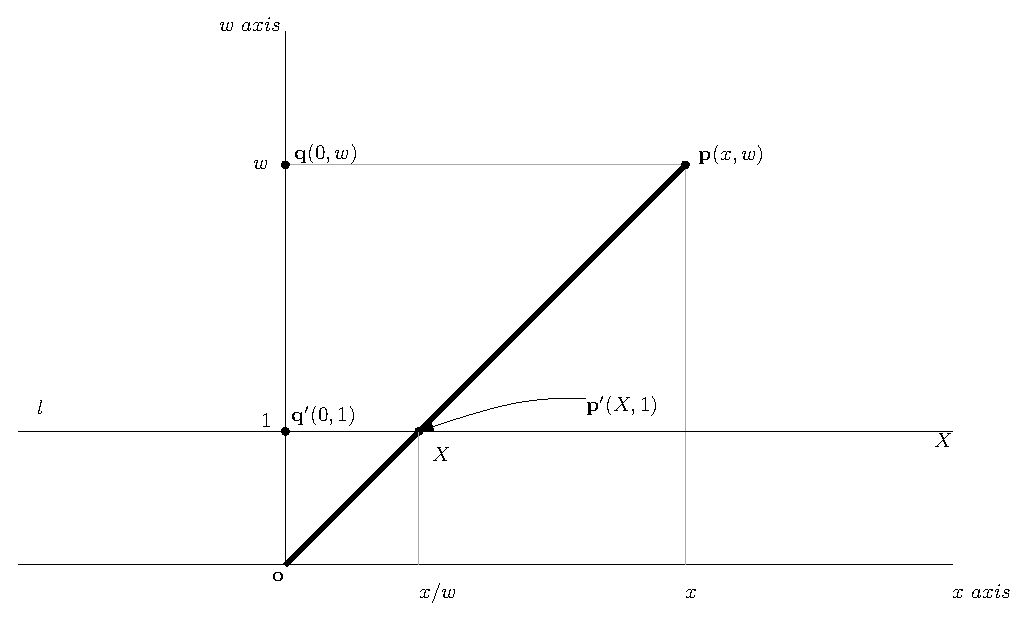
\includegraphics[width=12cm]{Math_transform/homogeneousConcept.eps}
\end{figure}

\end{frame}
%%%%%%%%%%%%%%%%%%%%%%%%%%%%%%%%%%%%%%%%%%%%%%%%%%%%%%%%%



%%%%%%%%%%%%%%%%%%%%%%%%%%%%%%%%%%%%%%%%%%%%%%%%%%%%%%%%%
\begin{frame}{동차좌표계의 시각적 이해 (2/2)}

\begin{itemize}
\item 두개의 축: $x$ 축이고, 다른 하나는 $w$ 축
	\begin{itemize}
	\item 동차 좌표계에서 마지막 원소 $w$를 제외한 모든 성분은 이 $x$ 축 값
	\item 마지막 원소는 이 $w$ 축 값
	\end{itemize}
\item $x$축 위에 있지 않는 점 $\mathbf p$는 중심 사영(central projection) $\mathbf p'$를 가짐
	\begin{itemize}
	\item $w=1$의 직선 $l$과 원점 $\mathbf o$에서 $\mathbf p$를 연결한 직선의 교차점
	\item 이때 원점은 사영중심(center of projection)
	\end{itemize}
\item $w$ 축과 $x$축을 모두 포함한 차원의 공간을 이보다 한 차원 낮은 $x$축 공간으로 떨어뜨리는 것
\item 선분 $\overline{\mathbf o \mathbf p}$를 지나는 직선 위의 모든 점들이 이 $\mathbf p'$로 사영
\item $(x,w)$에 해당하는 $\mathbf p'(X,1)$ 구하기
	\begin{itemize}
	\item 닮은 삼각형 $\mathbf{opq}$와 $\mathbf{op'q'}$
	\item 등비 관계를 이용하여 구한다
	\item $X = \frac{X}{1} = \frac{|\mathbf{p'q'}|}{|\mathbf{oq'}|}$
	\end{itemize}
\item 이 식은 다음과 같이 바뀐다.
\item $X = \frac{X}{1} = \frac{|\mathbf{oq'}|}{|\mathbf{p'q'}|} = \frac{|\mathbf{oq}|}{|\mathbf{pq}|} = \frac{x}{w} $
\end{itemize}



\end{frame}
%%%%%%%%%%%%%%%%%%%%%%%%%%%%%%%%%%%%%%%%%%%%%%%%%%%%%%%%%

%%%%%%%%%%%%%%%%%%%%%%%%%%%%%%%%%%%%%%%%%%%%%%%%%%%%%%%%%
\begin{frame}{동차좌표계와 데카르트 좌표계의 관계}

\begin{block}{$w$ 좌표의 의미}
사영기하에서 $\mathbf {op}$를 지나는 직선 위의 모든 점들은 $(x,w)$ 형태의 좌표로 표현할 수 있고,
이 모든 점들은 $w=1$인 평면으로 중심사영을 수행했을 때, $w$ 좌표는 무의미해지면서 $(x/w)$의 좌표로 바뀌게 된다.
즉, 3차원 공간의 좌표를 표현하기 위해 동차좌표계를 사용한다면 $[x,y,z,w]^{\rm T}$의 형태가 되며,
이것은 위의 그림에서 $w$ 축을 포함한 공간이 된다. 이를 3차원 데카르트 좌표로 바꾸는 것은 
중심사영이 이루어지는 $w=1$ 평면으로 옮겨 놓는 것이고 이때의 좌표는 $[x/w,y/w,z/w]^{\rm T}$가 되는 것이다.
그리고 3차원 공간의 측면에서 보면, $\mathbf {op}$를 지나는 직선 위의 모든 점들이 동일한 점으로 간주되는 것이다.
\end{block}

\end{frame}
%%%%%%%%%%%%%%%%%%%%%%%%%%%%%%%%%%%%%%%%%%%%%%%%%%%%%%%%%


%%%%%%%%%%%%%%%%%%%%%%%%%%%%%%%%%%%%%%%%%%%%%%%%%%%%%%%%%
\begin{frame}{동차 좌표계 사용의 이점(利點)}

\begin{itemize}
\item 3차원 좌표 $[x,y,z]^{\rm T}$를 동차좌표계 좌표로 바꾸는 간단한 방법은 $w=1$ 평면에서의 좌표인 $[x,y,z,1]^{\rm T}$
\item 동차좌표계를 쓰면 좋은 점
	\begin{itemize}
	\item 좌표와 벡터의 구분이 가능
	\item $[x,y,z]^{\rm T}$가 3차원 좌표라면 이 좌표로 표현되는 지점은 3차원 공간내 유일
	\item 벡터로 해석된다면 그것은 수 많은 동등 벡터를 표현하게 되며, 공간 내의 특별한 지점을 가리키지 않음
	\item 이 둘은 분명히 다르지만 단순한 좌표 표현 방식으로는 구분이 불가능
	\end{itemize}
\item 동차좌표계에서 좌표와 벡터의 구분
	\begin{itemize}
	\item 좌표는 $w \neq 0$인 $[x,y,z,w]^{\rm T}$
	\item 벡터는 $w = 0$인 $[x,y,z,0]^{\rm T}$
	\item $[x,y,z,0]^{\rm T}$는 위치를 가진 좌표 $[x,y,z]^{\rm T}$가 아니라 위치가 없는 벡터 $[x,y,z]^{\rm T}$
	\end{itemize}
\item 또다른 잇점
	\begin{itemize}
	\item 이동변환와 회전변환을 모두 같은 차원의 행렬로 표현
	\end{itemize}
\end{itemize}


\end{frame}
%%%%%%%%%%%%%%%%%%%%%%%%%%%%%%%%%%%%%%%%%%%%%%%%%%%%%%%%%

%%%%%%%%%%%%%%%%%%%%%%%%%%%%%%%%%%%%%%%%%%%%%%%%%%%%%%%%%
\begin{frame}{동차 좌표계에서 이동 변환}

동차좌표계에서의 이동

\begin{eqnarray}
\left [
\begin{array}{c}
x' \\y' \\ z' \\ 1
\end{array}
\right ]
=
\left [
\begin{array}{c}
x \\ y \\ z \\ 1
\end{array}
\right ]
+
\left [
\begin{array}{c}
d_x \\ d_y \\ d_z \\ 0
\end{array}
\right ]
=
\left [
\begin{array}{c}
x+d_x \\ y+d_y \\ z+d_z \\ 1
\end{array}
\right ] \nonumber
\end{eqnarray}


행렬 표현


\begin{eqnarray}
\left [
\begin{array}{c}
x' \\y' \\ z' \\ 1
\end{array}
\right ]
=
\left [
\begin{array}{cccc}
1 & 0 & 0 & d_x \\
0 & 1 & 0 & d_y \\
0 & 0 & 1 & d_z \\
0 & 0 & 0 & 1 \\
\end{array}
\right ]
\left [
\begin{array}{c}
x \\ y \\ z \\ 1
\end{array}
\right ]
=
\left [
\begin{array}{c}
x+d_x \\ y+d_y \\ z+d_z \\ 1
\end{array}
\right ] \nonumber
\end{eqnarray}


\end{frame}
%%%%%%%%%%%%%%%%%%%%%%%%%%%%%%%%%%%%%%%%%%%%%%%%%%%%%%%%%

%%%%%%%%%%%%%%%%%%%%%%%%%%%%%%%%%%%%%%%%%%%%%%%%%%%%%%%%%
\begin{frame}{이동 변환 행렬의 역행렬}

이제 이동변환을 행렬로 표현할 수 있게 되었다. 변위 벡터 $\mathbf d(d_x,d_y,d_z)$ 만큼의 이동을 수행하는 변환행렬을 $\mathbf T_{\mathbf d}$라고 하면
이동 변환은 다음과 같이 표현할 수 있다.

$$\mathbf p' = \mathbf T_{\mathbf d} \mathbf p, ~~~\mathbf T_{\mathbf d} \in \mathbb R^{4 \times 4}$$

이동변환 행렬 $\mathbf T_{\mathbf d}$의 역행렬은 어떻게 될까? 역행렬은 이 행렬이 일으킨 변환을 원래대로 되돌려 놓는 것이므로 
$\mathbf T_{- \mathbf d}$가 됨을 알 수 있다.

$$
\left [
\begin{array}{cccc}
1 & 0 & 0 & d_x \\
0 & 1 & 0 & d_y \\
0 & 0 & 1 & d_z \\
0 & 0 & 0 & 1 \\
\end{array}
\right ]^{-1}
= 
\left [
\begin{array}{cccc}
1 & 0 & 0 & -d_x \\
0 & 1 & 0 & -d_y \\
0 & 0 & 1 & -d_z \\
0 & 0 & 0 & 1 \\
\end{array}
\right ]
$$



\end{frame}
%%%%%%%%%%%%%%%%%%%%%%%%%%%%%%%%%%%%%%%%%%%%%%%%%%%%%%%%%


%%%%%%%%%%%%%%%%%%%%%%%%%%%%%%%%%%%%%%%%%%%%%%%%%%%%%%%%%
\begin{frame}{동차좌표계에서의 회전 행렬}

\begin{itemize}
\item 3차원 공간에서 정의되었던 회전 변환을 $\mathbf R_{33}$
\item $\mathbb R^{4 \times 4}$에 속하는 동차좌표계 회전 행렬은 $\mathbf R_{44}$
\item 원소가 모두 0인 3차원 열벡터를 $\mathbf O_3^{col}$, 행벡터를 $\mathbf O_3^{row}$
\end{itemize}

$$\mathbf R_{44} = 
\left [
\begin{array}{cc}
\mathbf R_{33} & \mathbf O_3^{col} \\
\mathbf O_3^{row} & 1
\end{array}
\right ]
$$

$
\mathbf R_{44}^x =
\left [
\begin{array}{cccc}
 1 & 0 & 0 & 0 \\
 0 & \cos \theta & -\sin \theta &  0\\
 0  & \sin \theta & cos \theta & 0 \\
 0 & 0 & 0 & 1 \\
\end{array}
\right ]
$
$
\mathbf R_{44}^y =
\left [
\begin{array}{cccc}
 \cos \theta & 0 & \sin \theta & 0 \\
 0 & 1 & 0 & 0 \\
- \sin \theta & 0  & \cos \theta & 0 \\
 0 & 0 & 0 & 1\\
\end{array}
\right ]
$

$$
\mathbf R_{44}^z =
\left [
\begin{array}{cccc}
 \cos \theta & - \sin \theta & 0 & 0 \\
 \sin \theta  & \cos \theta & 0 & 0 \\
 0 & 0 & 1 & 0 \\
 0 & 0 & 0 & 1\\
\end{array}
\right ]
$$



\end{frame}
%%%%%%%%%%%%%%%%%%%%%%%%%%%%%%%%%%%%%%%%%%%%%%%%%%%%%%%%%

%%%%%%%%%%%%%%%%%%%%%%%%%%%%%%%%%%%%%%%%%%%%%%%%%%%%%%%%%
\begin{frame}{복합변환}


좌표를 $\mathbf R_{44}$를 이용하여 회전하고, 이를 $\mathbf T_{\mathbf d}$ 만큼 이동하는 변환
\begin{eqnarray}
\mathbf p' = \mathbf T_{\mathbf d} \mathbf R_{44}  \mathbf p \nonumber
\end{eqnarray}

두 변환을 모두 수행하는 하나의 행렬 구할 수 있음 

\begin{eqnarray}
\mathbf p' & = &
\left [
\begin{array}{cc}
\mathbf I_{33} & \mathbf d \\
\mathbf O_3^{row} & 1
\end{array}
\right ]
\left [
\begin{array}{cc}
\mathbf R_{33} & \mathbf O_3^{col} \\
\mathbf O_3^{row} & 1
\end{array}
\right ]
\mathbf p \nonumber \\
& = &
\Large{
\left [
\begin{array}{cc}
\mathbf R_{33} & \mathbf d \\
\mathbf O_3^{row} & 1
\end{array}
\right ]
\mathbf p} \nonumber
\end{eqnarray}

\begin{itemize}
\item 행렬의 역행렬은?
\end{itemize}

\begin{eqnarray}
\left [
\begin{array}{cc}
\mathbf R_{33}^{\rm T} & \mathbf O_3^{col} \\
\mathbf O_3^{row} & 1
\end{array}
\right ]
\left [
\begin{array}{cc}
\mathbf I_{33} & - \mathbf d \\
\mathbf O_3^{row} & 1
\end{array}
\right ]
= 
\Large{
\left [
\begin{array}{cc}
\mathbf R_{33}^{\rm T} & - \mathbf R_{33}^{\rm T} \mathbf d \\
\mathbf O_3^{row} & 1
\end{array}
\right ]
} \nonumber
\end{eqnarray}

\end{frame}
%%%%%%%%%%%%%%%%%%%%%%%%%%%%%%%%%%%%%%%%%%%%%%%%%%%%%%%%%


%%%%%%%%%%%%%%%%%%%%%%%%%%%%%%%%%%%%%%%%%%%%%%%%%%%%%%%%%
\begin{frame}{복합변환}


좌표를 $\mathbf R_{44}$를 이용하여 회전하고, 이를 $\mathbf T_{\mathbf d}$ 만큼 이동하는 변환
\begin{eqnarray}
\mathbf p' = \mathbf T_{\mathbf d} \mathbf R_{44}  \mathbf p \nonumber
\end{eqnarray}

두 변환을 모두 수행하는 하나의 행렬 구할 수 있음 

\begin{eqnarray}
\mathbf p' & = &
\left [
\begin{array}{cc}
\mathbf I_{33} & \mathbf d \\
\mathbf O_3^{row} & 1
\end{array}
\right ]
\left [
\begin{array}{cc}
\mathbf R_{33} & \mathbf O_3^{col} \\
\mathbf O_3^{row} & 1
\end{array}
\right ]
\mathbf p \nonumber \\
& = &
\Large{
\left [
\begin{array}{cc}
\mathbf R_{33} & \mathbf d \\
\mathbf O_3^{row} & 1
\end{array}
\right ]
\mathbf p} \nonumber
\end{eqnarray}

\begin{itemize}
\item 행렬의 역행렬은?
\end{itemize}

\begin{eqnarray}
\left [
\begin{array}{cc}
\mathbf R_{33}^{\rm T} & \mathbf O_3^{col} \\
\mathbf O_3^{row} & 1
\end{array}
\right ]
\left [
\begin{array}{cc}
\mathbf I_{33} & - \mathbf d \\
\mathbf O_3^{row} & 1
\end{array}
\right ]
= 
\Large{
\left [
\begin{array}{cc}
\mathbf R_{33}^{\rm T} & - \mathbf R_{33}^{\rm T} \mathbf d \\
\mathbf O_3^{row} & 1
\end{array}
\right ]
} \nonumber
\end{eqnarray}

\end{frame}
%%%%%%%%%%%%%%%%%%%%%%%%%%%%%%%%%%%%%%%%%%%%%%%%%%%%%%%%%

%%%%%%%%%%%%%%%%%%%%%%%%%%%%%%%%%%%%%%%%%%%%%%%%%%%%%%%%%
\begin{frame}{좌표계의 변환}


\begin{itemize}
\item 어떤 점이 좌표계 $A$에 의해 $\mathbf p_A$라 표현된다고 가정
\item 다른 좌표계 $B$의 입장에서 보면 다른 좌표 $\mathbf p_B$
\item 이렇게 좌표계가 달라질 때 바뀐 좌표계에 따라 새로운 좌표를 계산하는 일은 그래픽스에서 매우 빈번히 나타나는 작업
	\begin{itemize}
	\item 가상 공간 내의 모든 객체의 위치를 하나의 기준으로 정의하는 데에 필요한 전역좌표계(global coordinate system)과 개별 객체 내에 정의된 지역좌표계(local coordinate system)
	\end{itemize}
\end{itemize}

\end{frame}
%%%%%%%%%%%%%%%%%%%%%%%%%%%%%%%%%%%%%%%%%%%%%%%%%%%%%%%%%

%%%%%%%%%%%%%%%%%%%%%%%%%%%%%%%%%%%%%%%%%%%%%%%%%%%%%%%%%
\begin{frame}[fragile]{좌표계의 이동}


$\mathbf p_A = \mathbf p_B + \mathbf d$
\begin{figure}
    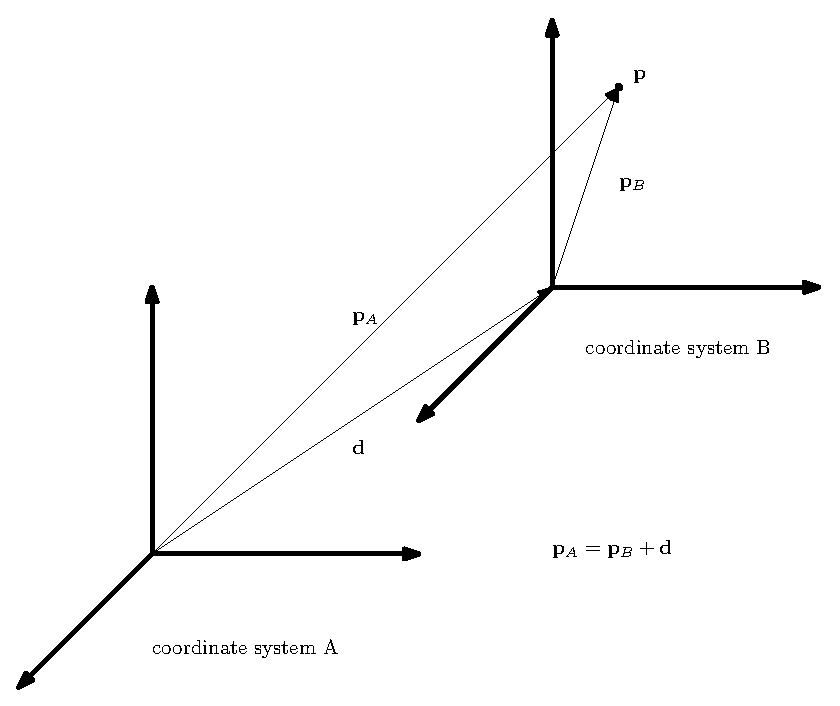
\includegraphics[width=6cm]{Math_transform/coordinateTranslate.eps}
\end{figure}

\begin{tabular}{lcc}
$
\mathbf T_{\mathbf d} = \left [
\begin{array}{cccc}
1 & 0 & 0 & d_x \\
0 & 1 & 0 & d_y \\
0 & 0 & 1 & d_z \\
0 & 0 & 0 & 1 \\
\end{array}
\right ],
$ &
$\mathbf p_A = \mathbf T_{\mathbf d} \mathbf p_B,$
&
$\mathbf p_B = \mathbf T_{\mathbf d}^{-1} \mathbf p_A$
\end{tabular}

\end{frame}
%%%%%%%%%%%%%%%%%%%%%%%%%%%%%%%%%%%%%%%%%%%%%%%%%%%%%%%%%

%%%%%%%%%%%%%%%%%%%%%%%%%%%%%%%%%%%%%%%%%%%%%%%%%%%%%%%%%
\begin{frame}[fragile]{좌표계의 회전}

\begin{eqnarray}
\mathbf p_A &= \mathbf R_{A \rightarrow B} \mathbf p_B & \nonumber \\
\mathbf p_B &=  \mathbf R_{A \rightarrow B}^{-1} \mathbf p_A & =  \mathbf R_{A \rightarrow B}^{\rm T} \mathbf p_A  \nonumber
\end{eqnarray}

\begin{figure}
    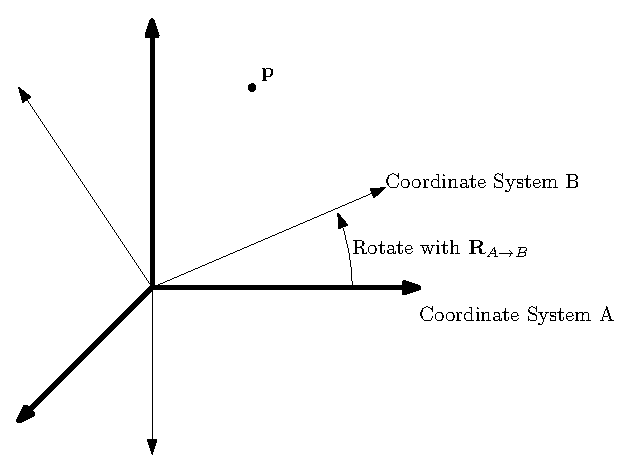
\includegraphics[width=8cm]{Math_transform/coordinateRotate.eps}
\end{figure}




\end{frame}
%%%%%%%%%%%%%%%%%%%%%%%%%%%%%%%%%%%%%%%%%%%%%%%%%%%%%%%%%

%%%%%%%%%%%%%%%%%%%%%%%%%%%%%%%%%%%%%%%%%%%%%%%%%%%%%%%%%
\begin{frame}[fragile]{회전과 이동이 함께 이뤄진 좌표계 변환 (1/2)}

\begin{figure}
    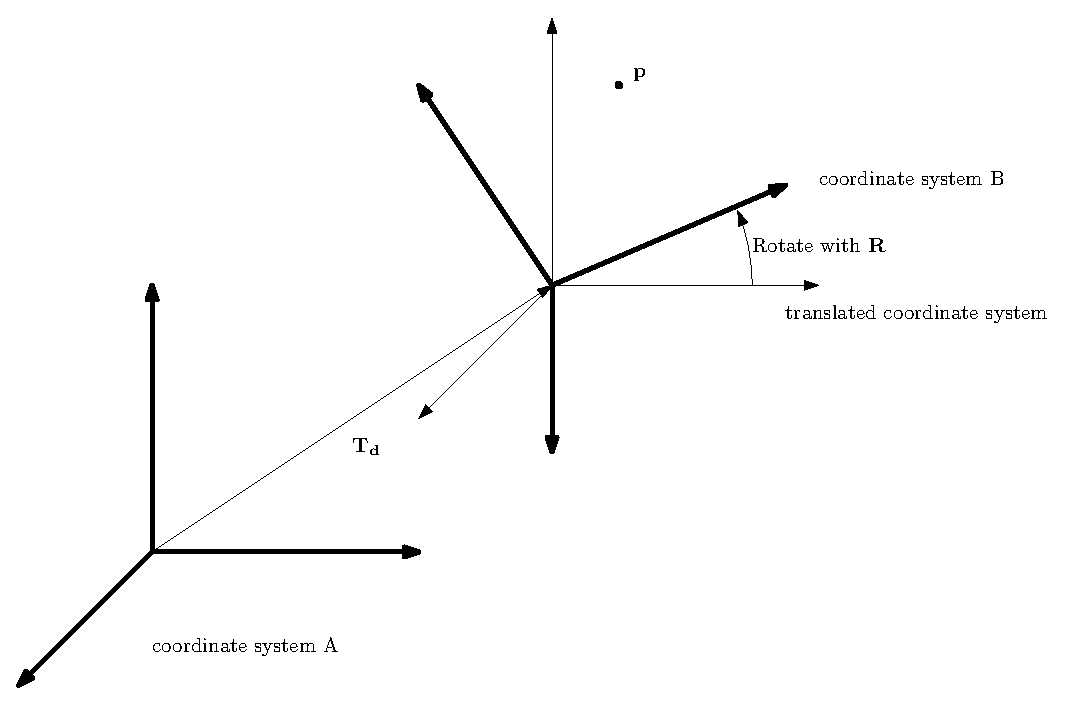
\includegraphics[width=10cm]{Math_transform/coordinateTransform.eps}
\end{figure}


\end{frame}
%%%%%%%%%%%%%%%%%%%%%%%%%%%%%%%%%%%%%%%%%%%%%%%%%%%%%%%%%

%%%%%%%%%%%%%%%%%%%%%%%%%%%%%%%%%%%%%%%%%%%%%%%%%%%%%%%%%
\begin{frame}[fragile]{회전과 이동이 함께 이뤄진 좌표계 변환 (1/2)}

$ 
\mathbf R = \left [ \begin{array}{cc} \mathbf R_{33} & 0 \\ \mathbf O_3^{row}  & 1 \end{array} \right ]
,~~~~$
$ 
\mathbf T_{\mathbf d} = \left [ \begin{array}{cc} \mathbf I_{33} & \mathbf d \\ \mathbf O_3^{row} & 1 \end{array} \right ]
,~~~~$
$ 
\mathbf T_{\mathbf d} \mathbf R = \left [ \begin{array}{cc} \mathbf R_{33} & \mathbf d \\ \mathbf O_3^{row} & 1 \end{array} \right ]
$


\begin{eqnarray}
\mathbf p_A &= 
\left [ \begin{array}{cc} \mathbf R_{33} & \mathbf d \\ \mathbf O_3^{row} & 1 \end{array} \right ]
\mathbf p_B & \nonumber \\
\mathbf p_B &=  
\left [ \begin{array}{cc} \mathbf R_{33}^{\rm T} &  \mathbf R_{33}^{\rm T} \mathbf d \\ \mathbf O_3^{row} & 1 \end{array} \right ]
\mathbf p_A  \nonumber
\end{eqnarray}

\end{frame}
%%%%%%%%%%%%%%%%%%%%%%%%%%%%%%%%%%%%%%%%%%%%%%%%%%%%%%%%%
